% 
%  chapter5.tex
%
\chapter{Implementation}\label{ch:implementation}

This chapter presents the solution developed to create CASCIFFO given the functional requirements detailed previously. It describes the techniques used and choices made throughout the implementation of the solution.

It is structured with the following sections:
\begin{itemize}
    \item Data modeling: Describes the data model used. 
    \item Back-end: Describes the back-end module.
    \item Front-end: Describes the front-end module.
    \item Continuous development: Usage of cloud-based platform Heroku for continuous development.
\end{itemize}

\section{Data modeling}~\label{sec:data-model}
In this section, a description of each entity that makes up the data model used for storing data on the CASCIFFO platform is provided, along with explanations of the reasons behind certain modeling decisions.
In this section, we introduce the data model, followed by the entities composing it.

\subsection{The data model}

The data model created to satisfy the needs of the platform CASCIFFO is centered around two main entities, firstly the Proposal entity which contains information regarding the submission and progress of a proposal of a clinical investigation. Secondly the Clinical Research entity which contains information pertaining to a clinical trial or clinical observation that has had its proposal submitted, accepted and validated.

A Proposal or Clinical Research entity can refer to either a clinical trial or observation study, depending on the field \textit{research\_type}. Although a clinical trial and an observational study are different, the information held by both is identical, differentiating only on existence of a financial component inherent to clinical trials. Therefore, these investigations can be stored regardless of their type in the mentioned entities. Aside from the identical data, another reason for choosing only one entity for representing clinical trials and observational studies in each stage, proposal submission and the active stage, is the amount of data stored, which is expected to be hundreds, so it makes it easier to do queries aimed at analyzing statistics.


\subsection{Proposal Entity}
Associated to a proposal entity is the type of service it's included in, the therapeutic area and type of pathology, these three fields correspond to a foreign key to their own entities. Each of these entities consist of two fields, an identifier and a name. They were made into entities rather than simple fields to allow for better consistency in the data model, since it makes use of built-in foreign-key validations and also facilitates creation and deletion of said fields. In addition to these fields, a proposal entity also has a principal investigator responsible for submitting the proposal, an investigation team with all the investigators that can edit the proposal, a set of Proposal Comments made within the scope of the proposal, a Financial Component in case its a proposal for a clinical trial, a set of timeline events and the files associated to the Proposal. 


\subsection{Clinical Research}
A clinical research has associated to it the proposal for which allowed for it to become active, a state indicating its current status, a list of visits that occur in the context of the investigation, a team of investigators, equal to the team submitted during its proposal stage and in case its a clinical trial it also has a financial component associated to it. It is to note that the financial component associated to a clinical research is different than a proposal's financial component. In addition, a clinical research can also have a list of several addenda.



\subsection{Addenda Entity}\label{subsec:addenda-entity}
The addenda entity, associated to a clinical research, can have a file associated to it pertaining to the change being made, a state since it must undergo a validation process before it has an affect on the clinical research and can have a list of comments.


\subsection{States}\label{subsec:states-entity}
The proposal, clinical research and addenda entity require state to track their evolution over time, thus the State entity was created, this entity holds all possible states for any proposal, clinical investigation or addenda. To differentiate between them an entity was created with the goal of interconnecting state chains. A state chain describes the flow from an initial state to a terminal state, i.e Proposal Submitted to Proposal Validated. 


\subsubsection{Next Possible States}\label{subsubsec:next-possible-states-entity}
This entity, called, Next Possible States, represents the possible transitions from one state to another, it contains two important fields that describe the chain the current state transition - \texttt{state\_type} - belongs to (i.e proposal, research or addenda), as well as the general order of the transition in the chain, initial for the first possible transition, progress for any in-between and terminal indicating the end of the chain.
To record the transitions, the entity State Transition was created, recording the previous state, new state, the date of transition, the type of transition (proposal, research or addenda) and finally the associated reference to what transitioned state. This reference is not a foreign key by choice, since it facilitates recording transitions in one entity rather than three different tables specifying the foreign relationship.


\subsubsection{Files}\label{subsubsec:files-model}
In addition to the need of tracking state, each of these entities can have their own resources in the form of files.
The files are stored on the operating system of the back-end module to avoid bloating the database with files, and only information about the full-path, file size, and name is stored in the database.


\section{Back-end module}\label{sec:back-end-module}
This section describes the summarized implementation choices of the Back-end module.
It first introduces the development of the back-end module and follows into more details regarding the repositories, services, controllers, mappers and authentication respectively.


\subsection{Back-end development}

The back-end module was developed using \textit{Spring Webflux}~\cite{spring-webflux} over Spring Web due to the reactive nature. \textit{Spring Webflux}~\cite{spring-webflux} brings a fully non-blocking programming environment and provides asynchronous calls to the database through the \textit{R2DBC} driver. This allows for a completely non-blocking experience from the moment an \textit{HTTP} request is received. 

The module consists of three layers, the Repository layer, which is responsible for database access, the Service layer, which is responsible for business logic, and finally the Controller layer, which receives and responds to requests. The layers communicate only with the layers below them, preventing circular dependencies. The controller layer communicates with the service layer, the service layer communicates with the repository layer and the latter communicates directly with the database. Across these layers there are exception handlers to handle any foreseen and unforeseen exceptions.

\subsection{Initial Development}

By using the tool \textit{Spring Initializr}~\cite{spring-io} provided by \textit{Spring} we're able to start with a project containing the necessary dependencies ready to launch. The project type was chosen to be Gradle-Kotlin, developed in Kotlin language, as illustrated in figure~\ref{fig:spring-io-start}.

\begin{figure}[H]
    \centering
    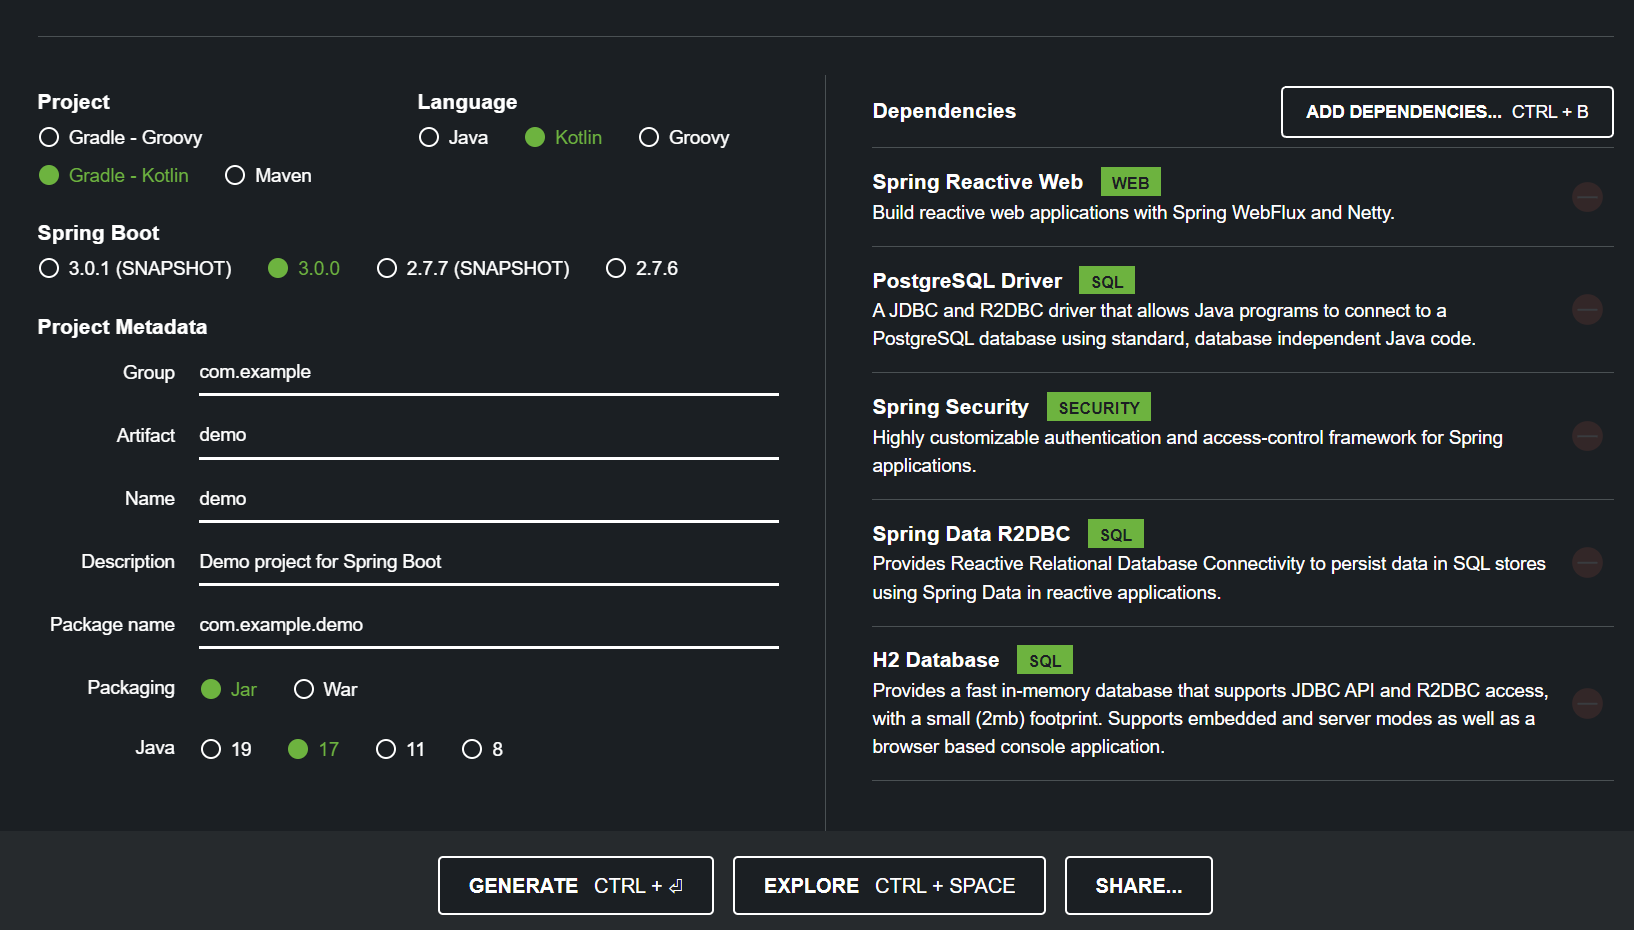
\includegraphics[scale=0.35]{Chapters/img/misc/spring-io.png}
    \caption{Initial project structure using \textit{Spring Initializr}~\cite{spring-io}.}
    \label{fig:spring-io-start}
\end{figure}

After downloading the project template, the project was organized by folders corresponding to each entity, this was chosen for the convenience of navigation due to the amount of entities.

In each entity folder, a class representing the controller, service and repository layer was created alongside the entity model itself.

\subsection{Repositories}\label{subsec:repositories}
The repository layer is responsible for directly accessing and manipulating data in the database. 

The repositories are interfaces annotated with Spring's \texttt{@Repository}, indicating they behave as a repository, each repository should implement an appropriate public interface, in the reactive context, it can either be \texttt{ReactiveCrudRepository} or \textit{ReactiveSortingRepository} followed by the type of entity and type of identifier (such as \texttt{ReactiveCrudRepository<Entity, EntityIdType}), where the former allows for basic CRUD operations (Create, Read, Update, Delete) without needing to implement further functionality, while the latter allows for built-in sorting functionalities. Spring also allows custom functions to be implemented either through naming conventions, such as \texttt{findAllByIdAndFieldIs(id, field)}, and through custom queries. For more complex queries another option is available, by annotating a method with \texttt{@Query(sql: String)} and passing a \texttt{string} argument with the SQL statement defined at design time. All repository methods should return a type encapsulated by either \texttt{Mono} or \texttt{Flux}. The type \texttt{Mono} should be returned when the method is expected to return between zero and a single result, while \texttt{Flux} should be used a result varying between zero and $n$ elements are expected. 

The entities used by repositories, in Kotlin, can be represented by data classes since they only contain data about the entity and have no behavior. 

A key factor to let the~\textit{Spring Webflux}ring~\cite{spring-webflux} framework know a data class is an entity, for the main purposes of saving and updating, is annotating said class with \texttt{@Table("table\_name")}, and the identifier field with \texttt{@Id}. It is worth noting that the identifier of a database table must be numeric. Text identifiers and compound keys don't function properly with this framework, so each database table has its own unique numeric identifier. 

When creating an entity, the property annotated with \texttt{@Id} must a value of \texttt{null}, otherwise, the framework will attempt to update an nonexistent entity. To work around this, we can either implement a custom repository and override the \texttt{save()} method or design the entities used to have an automatically generated identifier. The approach taken while building CASCIFFO's data model was the latter.

It should also be noted that naming conventions are taken into account between the database and the entity, the \textit{Snake Case} naming convention used by \textit{PostgreSQL}, is automatically converted into \textit{Camel Case} in \textit{Spring}, for example a table field named \texttt{created\_date} is automatically converted into \texttt{createdDate}.

One noticeable downside of using~\textit{Spring Webflux}~\cite{spring-webflux} and R2DBC, is that its current version doesn't provide mechanism of designing complex relationships with annotations, a feature available in \textit{Spring Web}. For example given two entities, A and B, with a relationship of 1-to-1, when fetching entity B, there isn't an automatic mechanism to build the associated entity A, after the fetch, the data will come as-is in the database, as opposed to \textit{Spring Data JPA} where such relationships can be modeled and built by the \textit{Spring Framework}. 
While nested entities can exist in a data class representing a database table, since they can't be loaded through automatic means, they must be annotated with \texttt{@Transient} alongside \texttt{@Value(defaultValue)}. 
The former annotation tells \textit{Spring}'s framework to ignore the annotated property when saving a new entity while the latter annotation comes into play during the mapping after a fetch, this annotation defines the default value to assign to the annotated property, in the development context, the value assigned was always \texttt{@Value("null")}. 

This means that for complex entities with multiple foreign keys, with each foreign key corresponding to a nested object that needs to be manually instantiated, in order to fetch the data to build these objects would require to make that as database calls as there are nested entities which leads to performance issues. To counter this, entities were created to serve as containers of data, by aggregating all the fields required to build not only the base entity but also the nested ones. 
In conjunction with this, for each of these containers a repository was created, however, since the data that we want is split between tables, a custom query is needed to fetch the desired results. By using this approach we can specify all the necessary data manually. On a side note the aggregate entity doesn't need to be annotated with \texttt{@Table()} since it will exclusively used for fetching data.


\subsection{Services}

The service layer is where all business logic is handled. The approach taken to implement this layer was with interfaces together with Spring's dependency injection, all services have an interface that describes their operations. The implementation of these services must then be annotated with @Component so Spring can easily scan and auto inject the implementations to where they're used. This facilities maintenance and rearranging of code, as well as building and swapping existing implementations of a service.

Each service can communicate with other services and with their associated repositories, in addition to business logic, the request parameter validation and other exceptions are thrown and handled in this layer.

\subsection{Controllers}

The controller layer is where the \textit{HTTPS} requests are handled, the routing of requests is handled by Spring's framework with the help of annotations that distinguish what controller handles which route and operation.
To build a controller class, the class needs to be annotated with \texttt{@Controller} or in this case of a \textit{REST API} module, \texttt{@RestController}. The main difference between the two annotations is that \texttt{@RestController} indicates that the class is a controller where \texttt{@RequestMapping} methods assume \texttt{@ResponseBody} semantics by default.
The \texttt{@RequestMapping} accepts a route path to serve as the base of the controller class, \texttt{@ResponseBody} indicates the type of response, in this case, \texttt{JSON} is used in all responses. 

When building the operations of a controller class, the methods that handle route requests, depending on the type of operation, need to be annotated with one of the following \texttt{@Post}, \texttt{@Put}, \texttt{@Get}, \texttt{@Patch} or \texttt{@Delete}, each of these annotations take in an optional argument that represents the path of the route taking into account the base path if specified in \texttt{@RequestMapping(path)} on the class. 

Each of the methods in a controller class can return an object or a \texttt{ResponseEntity<Type>} for more flexibility in the structure of the response. In the reactive environment that\textit{Spring Webflux}~\cite{spring-webflux} provides, each return type should be inside a \texttt{Mono} or \texttt{Flux} stream.
The former represents a stream of one object, whereas the latter a stream of objects, from 0 to N objects. \texttt{Mono} and \texttt{Flux} represent streams of data using \textit{Reactor}, these data types can be chained together like building blocks in a declarative manner of programming. First the developer explicitly declares the behavior of the chain, with functions such as \texttt{map(), filter(), groupBy(), flatMap()}. The execution of this chain only begins once the stream is subscribed to. 

Returning a \texttt{Mono} or \texttt{Flux} lets the Spring framework handle when its subscribed and structures the response data, whenever a conversion to \texttt{JSON} happens the streams are automatically subscribed to.
While \texttt{Mono} and \texttt{Flux} are \textit{Spring Webflux}~\cite{spring-webflux}'s standard since it operates over \textit{Reactor}, \textit{Kotlin} also offers another way of dealing with streams, while implementing the back-end module \textit{Kotlin Coroutines}~\cite{kotlin-coroutines} were preferred over \texttt{Mono} and \texttt{Flux} due to its \texttt{async-await} nature and ease of use. To use \textit{Kotlin Co-routines} the functions need to have the \texttt{suspend} keyword, i.e \texttt{suspend fun functionName(params)}, in this way, instead of returning a \texttt{Mono<Type>} we can return the \texttt{Type} directly. When dealing with \texttt{Flux} data types, \textit{Kotlin} offers an alternative called \texttt{Flow<Type>}, the type \texttt{Flow} has a similar set of operations and behavior to \texttt{Flux}. To convert a stream of type \texttt{Flux} to a \texttt{Flow}, a simple call to the method \texttt{asFlow()} applied to the \texttt{Flux} stream will do the job.

A caveat of \texttt{Flux} and \texttt{Flow} occurs when returning objects with nested streams, (i.e returning a \texttt{Flow} of object A that has a nested \texttt{Flow} of object B in its instance), during \textit{Spring}'s automatic conversion from object to \texttt{JSON}, the nested streams aren't represented properly, showing only a fetch status instead of the stream itself. In order to address this issue, a \acrfull{dto} representation of each entity model was created to hold lists instead of reactive streams. In conjunction with this, several mappers were created for the conversion of entity models to their respective DTO representations.


\subsubsection{Mono/Flux syntax vs Suspend function syntax}~\label{subsubsec:kotlin-coroutines}

To understand the concept of a suspend function we must first understand what are \textit{Kotlin coroutines}, since a suspend function is a coroutine itself.

A \textit{Kotlin coroutine}, taken to its literal name, co and routine, can be seen as a cooperative routine, meaning a conjunction of instructions (routine) that runs along (co) with other tasks. In other words, a coroutine is an instance of suspendable computation that can execute blocks of code in concurrency with other coroutines.
In the context of concurrent programming, we find another and very common way of of dealing with concurrent tasks; threads. 

\textit{Kotlin coroutines} and threads are both ways of concurrent programming, but they have some significant differences.
A coroutine is conceptually similar to a thread, in the sense that it takes a block of code to run concurrently with the rest of the code. However, a coroutine is not bound to any particular thread. It may suspend its execution in one thread and resume in another one.~\cite{kotlin-coroutines-your-first}

According to the article by~\citename{kotlin-lightweight}{author} of the main differences between coroutines and threads is that coroutines are light-weight, while threads are heavy-weight. This means that coroutines use much less memory and computational resources than threads, and can therefore be more efficient when dealing with large numbers of concurrent tasks.

Another difference pointed out in the same article, is that coroutines are cooperatively scheduled, while threads are preemptively scheduled. This means that in a coroutine, the currently running coroutine must explicitly yield control to another coroutine, while in a thread, the scheduler can interrupt the currently running thread at any time and give control to another thread. We can say that unlike threads which are usually controlled by the operating system, coroutines are managed by the user in conjunction with the programming language. This makes coroutines easier to reason about and debug, because the control flow is more predictable.

Additionally, coroutines can be easily composed and used in a non-blocking manner, while threads require explicit synchronization mechanisms such as locks or semaphores to avoid race conditions and deadlocks.

Overall, coroutines are a more modern and efficient way of concurrent programming.

% 
% Here are some references that provide more information about the differences between Kotlin coroutines and threads:

% The Kotlin coroutines documentation, which explains the basics of coroutines and how they compare to threads: https://kotlinlang.org/docs/reference/coroutines/coroutines-guide.html
% This article, which provides a detailed comparison of coroutines and threads in Kotlin: https://proandroiddev.com/kotlin-coroutines-vs-threads-847b0e6e77c6
% This video, which discusses the differences between coroutines and threads and provides some examples of using coroutines in Kotlin: https://www.youtube.com/watch?v=_hfBv0a09Jc
% 
Now that the concept of a \textit{Kotlin coroutine} has been 
To define a coroutine function, we simply need to add the keyword \texttt{suspend} before the declaration of the function thus making it a \textit{suspending} function.

On the topic of syntax choice, \textit{Kotlin Coroutines}~\cite{kotlin-coroutines} was favored due to the simplicity and clarity of the written code.
To illustrate the difference in syntax between the usage of \textit{Spring}'s \texttt{Mono}/\texttt{Flux} and \textit{Kotlin coroutines} we'll use a small portion of CASCIFFO's data model focusing on a proposal, its principal investigator and the states of a proposal. The entities in play will be \texttt{Proposal}, \texttt{User} - representing investigators - and \texttt{Comment}. Following the context given, a proposal has one principal investigator and can have several comments made by other investigators. The data of a proposal is split in the database, when wanting to get the full details of a proposal, a query must also be made to fetch the \texttt{User} and another to fetch the~\texttt{Comment} associated to the proposal. Assuming a repository exists for each of these entities their names are their respective entities suffixed with \texttt{Repo} we can write the following code to query the database and fetch the entities needed to build a proposal with nested entity of investigator and a list of comments.
Below is the representation of the method \texttt{getProposalDetails} using \texttt{Mono}/\texttt{Flux} in listing~\ref{lst:mono-syntax} and using a \textit{Kotlin Coroutine} in listing~\ref{lst:suspend-syntax}.

\begin{lstlisting}[
    language=kt, 
    caption={Loading nested entities in an object using Mono/Flux syntax}, 
    label={lst:mono-syntax}
]
fun getProposalDetails(pId: Int): Mono<Proposal> {
    return personRepo
        //findById returns Mono<Proposal>
        .findById(pId) 
        // zipWith returns Mono<Tuple2<Proposal, User>>
        .zipWith(userRepo.findByProposalId(pId)) 
        .flatMap{ 
            it.t1.pInvestigator = it.t2.get()
            it.t1 //Proposal
        }
        // zipWith returns Mono<Tuple2<Proposal, (Mutable)List<Comment>>
        .zipWith(commentsRepo.findAllByProposalId(pId).collectList()) 
        .flatMap {
            it.t1.comments = it.t2.get().map{e ->  commentsMapper.mapToDto(e) }
            it.t1
        }
}    
\end{lstlisting}


\begin{lstlisting}[
    language=kt, 
    caption={Loading nested entities in an object using suspend function syntax},
    label={lst:suspend-syntax}]
suspend fun getProposalDetails(pId: Int): Person {
    val proposal = proposalRepo.findById(pId).awaitSingle()
    person.pInvestigator = userRepo.findByProposalId(pId).awaitSingle()
    //here comments was changed from type Flux<Comment> to Flow<Comment>
    person.comments = commentsRepo.findAllByPersonId(pId).asFlow()
    return proposal
}    
\end{lstlisting}


\subsection{Mappers}

Mappers are crucial tool in any application, allowing the conversion of one data type into another and hiding the complexity of such operation. Using Spring's powerful dependency injection a single generic \texttt{Mapper<ModelType, DTOType>} interface was created with the methods \texttt{mapDTOtoModel()} and \texttt{mapModelToDTO()}, both methods are suspend functions.
During the mapping phase, nested objects of type \texttt{Flux} or \texttt{Flow} are subscribed to and subsequently transformed into lists that can be represented in \textit{JSON}.

Each mapping conversion from DTO to Model and vice versa are called within the controllers.


\subsection{Authentication}

On top of these layers lies Spring's own framework, and in it the Web Filters. Web Filters are methods that run during an incoming request. Through Spring's framework, they intercept and perform operations with the request data before control is given to a controller handler. 
These Web Filters are especially useful to perform authentication operations on the incoming requests.


The authentication was implemented with \acrfull{jwt}, each request that requires authentication must have a valid \acrshort{jwt} in the header 'Authentication' of the request. This \acrshort{jwt} in addition to the standard fields, also holds user information, namely the user email that is used to uniquely identify each user. 
To further security, a role-based access control was defined as mentioned previously in the document. This can be implemented in a few steps, first and foremost is to implement\textit{Spring Webflux}~\cite{spring-webflux}'s \texttt{ReactiveUserDetailsService}, which is responsible for fetching a user based on a passed argument \texttt{username}, this method will be called during the interception of a request that requires authentication. The next step is to create an authentication manager that implements \texttt{ReactiveAuthenticationManager} and overriding the method \texttt{authenticate}, this manager is responsible for extracting and validating the information from a \acrshort{jwt}. Note that both the classes that implement these interfaces need to be annotated with \texttt{@Component}. The need for the annotations comes from a useful feature of \textit{Spring}'s framework, dependency injection, by annotating these classes with \texttt{@Component} or methods with \texttt{@Bean} allows \textit{Spring} to scan and detect the classes and auto inject them into other parts of the code where they are passed as arguments for methods or constructors. \textit{Spring} taking control of this aspect of the code, can be referred as \acrfull{ioc} where a framework takes control of a portion of the program or code, instead of the programmer explicitly controlling it.
 
To make use of this newly created components we need to add the authentication manager to the \texttt{WebFilter} chain that can be accessed and configurable from a class annotated with \texttt{@Configuration} and implementing the method \texttt{springSecurityFilterChain}, annotated with \texttt{@Bean}. 
This method receives an argument \texttt{http} of type \texttt{ServerHttpSecurity} and should also receive the created authentication manager component as an argument. 
Finally to add it to the \texttt{WebFilter} chain, the method \texttt{addFilterAt()} is used, applied to the argument \texttt{http}. 

This describes how a \acrshort{jwt}'s information is extracted and validated, to implement a role-based access control, one can choose Spring's annotation-based authentication, by annotating the required methods or controller classes with \texttt{@PreAuthorize(string)}. The passed argument is a function name alongside its arguments, in this context, the most adequate ones would be \texttt{hasAuthority()} or \texttt{hasAnyAuthority()}. Another possible way of implementing this requirement is by utilizing the \texttt{http} argument mentioned previously inside the method \texttt{springSecurityFilterChain} and programmatically add these rules to each route, as shown in the coding listing~\ref{lst:spring-security}. By utilizing the methods \texttt{authorizeExchange()} followed by \texttt{pathMatchers(route)} and applying \texttt{hasAnyAuthority(authorities)} or \texttt{hasAuthority(authority)}. An authority is simply a constant with a string value specifying a role, for context, some of the authorities used were \texttt{SUPERUSER\_AUTHORITY} and \texttt{UIC\_AUTHORITY}. 


\begin{lstlisting}[
    language=kt, 
    caption={Configuration of spring security filter chain},
    label={lst:spring-security}]
@Bean
fun springSecurityFilterChain(
    converter: JwtServerAuthenticationConverter,
    http: ServerHttpSecurity,
    authManager: JwtAuthenticationManager
): SecurityWebFilterChain {

    val jwtFilter = AuthenticationWebFilter(authManager)
    jwtFilter.setServerAuthenticationConverter(converter)

    http
        .addFilterAt(jwtFilter, SecurityWebFiltersOrder.AUTHENTICATION)

    //example of routing configuration
    http
        .authorizeExchange()
        .pathMatchers(HttpMethod.GET, ENDPOINTS_URL)
            .permitAll()
        .pathMatchers(HttpMethod.POST, ENDPOINTS_URL)
            .hasAnyAuthority(SUPERUSER_AUTHORITY, UIC_AUTHORITY)
        .pathMatchers(HttpMethod.DELETE, ENDPOINTS_URL)
            .hasAuthority(SUPERUSER_AUTHORITY)
             
    //other http configurations
    ...
            
    return http.build()
}
\end{lstlisting}

Both the discussed approaches were used, having settled with programmatically adding new rules to the routes themselves. This choice was made based on performance issues with the annotation-based authentication, the annotation \texttt{@PreAuthorize()} was adding an overhead of up to 1 second per request, whereas programmatically this issue was not observed. The cause can be due to\textit{Spring Webflux}~\cite{spring-webflux}, since the annotation \texttt{@PreAuthorize} is more commonly used with Spring Web.


\subsection{Exception handling}

On the topic of business rules, once one is broken, an exception is raised with information regarding the cause. Business rules are defined in the service layer and conversely it is where incoming requests are validated before performing the requested process. If the information passed along the request isn't valid, an exception is manually thrown with an appropriate \texttt{HTTP status} and a reason, since the back-end module exposes an API through http requests. 

With exceptions being raised whenever there's invalid data on incoming requests, the response must come with appropriate information on why the request failed or was rejected. For example, when requesting a resource that requires authentication yet the request sent none, the response will provide sufficient information so the one that made the request knows that for accessing that specific resource, it is also required to send authentication and how to send it.

To handle these exceptions and others that can occur during run-time, such as a database integrity violation or in case the database is unreachable among other possible run-time exceptions we can make use of great features provided by \textit{Spring}'s framework. We first looked at utilizing custom exceptions annotated with \texttt{@ResponseStatus}, by annotating a class that extends \texttt{Exception}, we can define the response status code and the reason that caused the exception to be thrown, as illustrated by the listing~\ref{lst:ex-rsp-status}. 

\begin{lstlisting}[
    language=kt,
    label={lst:ex-rsp-status},
    caption={Example of an exception annotated with @ResponseStatus}
]
@ResponseStatus(
    code = HttpStatus.NOT_FOUND, 
    reason = "Specified resource Id doesn't exist."
)
class ResourceNotFoundException(): Exception()
\end{lstlisting}

This approach is simple and makes use of \textit{Spring}'s automatic converter to \textit{JSON}. The issue lies in its simplicity, it doesn't allow us to change anything other than reason and status code, the body itself is handled by \textit{Spring}, an example of an answer can be observed in the code listing~\ref{lst:ex-response-example}. 
We would also need to create several exception classes for each edge case that requires an exception to be thrown.

\begin{lstlisting}[
    language=json,
    label={lst:ex-response-example},
    caption={Example response using \textit{Spring}'s automatic response converter.}
]
"{
    "timestamp": "2022-11-09T12:24:21.609+00:00",
    "path": "/proposals/999",
    "status": 404,
    "error": "Not Found",
    "message": "Specified resource Id doesn't exist.",
    "requestId": "c0d35eab-2"
}"
\end{lstlisting}


One other possible solution was to create specific exception handlers, using the annotation \texttt{@ExceptionHandler(SampleException::class)} on a method and passing the class type of exception to catch as its argument, we can process specific exceptions locally within the controller classes themselves. This resolves issue of the first approach in the sense that we can make use of the incoming request and outgoing response to write our own defined response body. 
The trade offs, however, come at a cost of maintenance, the exception handlers will be tightly coupled to their controllers and one exception handler can only process one type of exception.

Another analyzed approach was the implementation of \texttt{ErrorWebExceptionHandler} and overriding the method \texttt{override fun handle(ServerWebExchange, Throwable): Mono<Void>}. The purpose of this method is to catch any exceptions not handled by the exception handlers mentioned earlier. In the context of this method we have access to the argument of type \texttt{ServerWebExchange} which includes in its properties the request, the response and other useful information about the this particular connection that resulted in an exception. Here we are also able to access and customize the body property of the response as we wish.

Yet another studied approach was the usage of classes annotated with \texttt{@RestControllerAdvice}, these classes can intercept exceptions when controllers, respectively annotated with \texttt{@RestController} raise exceptions. With this class we can centralize all exception handlers in one place, decoupling the controllers of their exception handlers and moving the latter here. 

The last studied solution was the usage of the exception class  \texttt{ResponseStatusException}, which on the contrary to the first mentioned approach, we define raise the exceptions and set their status and reason locally when the exception is thrown. This reduces the amount of exception classes since one type of exception can be used for any issue which great for prototyping and testing. A trade off of this approach will be the increased difficulty of code management and duplicated code inside the code blocks that raise exceptions. 

The final solution taken was a mix and match of the described approaches. A global exception handler was created by utilizing the creation of a class annotated with \texttt{@RestControllerAdvice} and implementing \texttt{ErrorWebExceptionHandler} to catch any unexpected exception during run-time. For specific exceptions, the usage of a method annotated with \texttt{@ExceptionHandler} and accepting the argument \texttt{ResponseStatusException::class} facilitated in manipulating the response body. With this solution, we benefit from global exception handling and decoupled controllers.


\section{Front-end module}

The \acrshort{fe} module was developed using \textit{ReactJs}~\cite{reactjs}, version 18, mainly due to its popularity and ease of use alongside a super set of \textit{JavaScript}; \textit{TypeScript}, version 4. The module is built using a node package manager, the popular \textit{npm}~\cite{npm}, and deployed with \textit{npx webpack} during development. 

This module was developed to be a \acrfull{spa} and consists of three main components, the View, Model and Service.

Starting from the service component, this is where data is requested via \textit{HTTPS} to the back-end module.
All services are stateless and responsible for requesting data.

The model component is where all model entities are held. 

Finally the view component is where the magic happens, the business logic of the \acrfull{fe} module is near the client and occurs within each Component depending on its responsibility.
In \textit{ReactJs}~\cite{reactjs}, the \acrshort{ui} is built with components, each component can be viewed as a building block of a page, it is reusable and provides ways to handle state and logic.

Moving to security in the front-end module, role based access-control is a requirement, in order to satisfy this, a login system was developed using the concept of \acrfull{hoc}, these components are the same as any other, however, they have the responsibility to perform validations before rendering other components. To implement this functionality, any page that requires a user being authenticated or having a specific role will be chained with a \acrshort{hoc}, first the \acrshort{hoc} is rendered, which performs validations on the user info available on the browser session storage and makes a decision on whether to render the page requested or display an error.
Upon a successful login, the back-end module sends a valid \acrshort{jwt}, the user identifier and the roles associated to the logged in user that is then stored within the browser's session storage.

According to the functional requirements the screens were developed based on the mock ups detailed in the report. In addition, the module follows the standard of a \acrfull{pwa}, allowing the application to be downloaded from the browser, to work as a mobile app and offline functionality albeit limited. The dashboard screen currently displays several useful stats through graphs and tables.

Each page corresponds to a route that is handled by \textit{React.Router}, however, during development an issue arouse which was when accessing an \texttt{URL} other than base one first such as, \texttt{[base-path]/propostas} instead of \texttt{[base-path]}, it displayed the error \texttt{Cannot GET [URL]}, this issue was due to how \textit{React.Router} interacts with the \texttt{URL}.
\textit{React.Router} is only loaded when the base \texttt{URL} is first called, after which it takes control of the route handling. To resolve this, a simple line of code was needed to be added to the server start up file, which redirects any all \texttt{URL} requests to the base path first and foremost. This way, \textit{React.Router} is always loaded and becomes capable of handling requests as expected.


\section{Heroku Deployment}

The approach to the development of CASCIFFO involved a technique of continuous development and testing, this was possible by deploying both modules to the cloud platform Heroku and having them available for testing. With each new feature a new deployment was released without compromising having the this testing environment go down while working on new features. 

\section{On-Premises Deployment}

\subsection{Installing PostgreSQL}
\subsection{Installing Java}
\subsection{Installing Node}
\subsection{Deploying the Application}
\subsection{Apache Hosting}
\subsubsection{Configuration}
\subsubsection{Modules}
\subsubsection{Verifying Hosted Application}